\documentclass[wabun2025.tex]{subfiles}
\begin{document}
\appendix
\section{Derivation of the Effective Radius for the Local Average Potential}
\label{chap:appendix_derivation_derivation}
\subsection{Derivation from the Equivalence of Energy Expectation Values}
We present the derivation of the parameter $\reff$ in the approximation formula
$\Hla(r)$ described in Section \ref{sec:coulomb-potential-handling}.

First, the derivation of Equation \eqref{eq:delta-1-0-0} regarding
$\PsiTwoD_{0,0}$ is shown.

The integral $W_{0,0}$ is given by,
\begin{align}
  W_{0,0}
   &= \int_{\theta=0}^{2\pi}d\theta
      \int_{r=0}^{\deltar/2}
      \Hep(r)\abs{\PsiTwoD_{0,0}(r)}^2r dr\notag\\
   &= 2\pi
      \int_{r=0}^{\deltar/2}
      -\frac{1}{r}\left(\frac{q_0^3(0-\abs{0})!}{\pi(0+\abs{0})!}\right)
      (2q_0r)^{2\abs{0}}\exp(-2q_0r)
      \left[L_{0-\abs{0}}^{2\abs{0}}(2q_0r)\right]^2 r dr\notag\\
   &= -2\pi\int_{r=0}^{\deltar/2}\frac{q_0^3}{\pi}\frac{1}{r}e^{-2q_0r}r\ dr=-2q_0^3
      \left[-\frac{1}{2q_0}e^{-2q_0r}\right]_{0}^{\deltar/2}\notag\\
   &=-q_0^2(-e^{-q_0\deltar}+1)
\end{align}
On the other hand, $W_{0,0}^\prime$ is given by,
\begin{align}
    W_{0,0}^\prime
    &=\pi\left(\frac{\deltar}{2}\right)^2
       \Hla(0)\abs{\PsiTwoD_{0,0}(0)}^2\notag\\
    &=\frac{\pi\deltar^2}{4}\left(-\frac{1}{\reff}\right)
    \left(\frac{q_0^3(0-\abs{0})!}{\pi(0+\abs{0})!}\right)
    (0)^{2\abs{0}}\exp(0)\left[L_{0-\abs{0}}^{2\abs{0}}(0)\right]^2\notag\\
    &= -\frac{\pi\deltar^2q_0^3}{4\pi\reff}\notag\\
    &= -\frac{\deltar^2q_0^3}{4\reff}
\end{align}
Solving $W_{0,0}=W_{0,0}^\prime$ yields,
\begin{equation}
-q_0^2\left(-e^{-q_0\deltar}+1\right)=-\frac{\deltar^2q_0^3}{4\reff}
\end{equation}
\begin{align}
\reff&=\frac{\deltar^2q_0}{4\left(-e^{-q_0\deltar}+1\right)}\notag\\
&\simeq\frac{\deltar^2q_0}{4\left(-(1-q_0\deltar)+1\right)}\notag\\
&=\frac{\deltar}{4}
\end{align}

Next, the derivation of Equation \eqref{eq:delta-1-1-0} regarding $\PsiTwoD_{1,0}$ is shown.

Calculating $W_{1,0}$ and $W_{1,0}^\prime$ respectively, $W_{1,0}$ is given by,
\begin{align}
  W_{1,0}
   &= \int_{\theta=0}^{2\pi}d\theta
      \int_{r=0}^{\deltar/2}\Hep(r)\abs{\PsiTwoD_{1,0}(r)}^2r dr\notag\\
   &= 2\pi\int_{r=0}^{\deltar/2}
      -\frac{1}{r}\left(\frac{q_0^3(1-\abs{0})!}{\pi(1+\abs{0})!}\right)
      (2q_0r)^{2\abs{0}}\exp(-2q_0r)
      \left[L_{1-\abs{0}}^{2\abs{0}}(2q_0r)\right]^2 rd\theta dr\notag\\
   &= -2\pi\int_{r=0}^{\deltar/2}\frac{q_0^3}{\pi}e^{-2q_0r}(1-2q_0r)^2dr\notag\\
   &= -2q_0^3\left[\left(-\frac{1}{2q_0}+2q_0r^2\right)e^{-2q_0r}\right]_{0}^{\deltar/2} \notag\\
   &= -2q_0^3\left\{\left(-\frac{1}{2q_0}+\frac{q_0\deltar^2}{2}\right)e^{-q_0\deltar}+\frac{1}{2q_0}\right\}\notag\\
   &= q_0^2\left\{\left(1-q_0^2\deltar^2\right)e^{-q_0\deltar}-1\right\}
\end{align}
On the other hand, $W_{1,0}^\prime$ is given by,
\begin{align}
    W_{1,0}^\prime
    &=\pi\left(\frac{\deltar}{2}\right)^2
         \Hla(0)\abs{\PsiTwoD_{1,0}(0)}^2\notag\\
    &=\frac{\pi\deltar^2}{4}\left(-\frac{1}{\reff}\right)
    \left(\frac{q_0^3(1-\abs{0})!}{\pi(1+\abs{0})!}\right)
    (0)^{2\abs{0}}\exp(0)\left[L_{1-\abs{0}}^{2\abs{0}}(0)\right]^2\notag\\
    &= -\frac{\pi\deltar^2q_0^3}{4\pi\reff}\notag\\
    &= -\frac{\deltar^2q_0^3}{4\reff}
\end{align}
Solving $W_{1,0}=W_{1,0}^\prime$ yields,
\begin{equation}
q_0^2\left\{\left(1-q_0^2\deltar^2\right)e^{-q_0\deltar}-1\right\}
=-\frac{\deltar^2q_0^3}{4\reff}
\end{equation}
\begin{align}
\reff&=\frac{\deltar^2q_0}{4\left\{\left(1-q_0^2\deltar^2\right)e^{-q_0\deltar}-1\right\}}\notag\\
&\simeq-\frac{\deltar^2q_0}{4\left\{\left(1-q_0^2\deltar^2\right)(1-q_0\deltar)-1\right\}}\notag\\
&=-\frac{\deltar^2q_0}{4\left(1-q_0^2\deltar^2-q_0\deltar+q_0^3\deltar^3-1\right)}\notag\\
&\simeq\frac{\deltar}{4}
\end{align}
is obtained.

\subsection{Derivation from the Geometric Average}
The derivation of the parameter $\reff$ in the approximation formula $\Hla(r)$
described in Section \ref{sec:coulomb-potential-handling} is shown using a
method that determines it from the simple geometric average of the potential in
a minute circular region centered on the singularity of the Coulomb potential.
The geometric average of the potential in a circular region of radius
$R=\deltar/2$ centered on the singularity of the Coulomb potential is given by,
\begin{align}
    \bar{V} &= \frac{1}{\pi R^2}\int_{r=0}^{R} -\frac{1}{r} 2\pi r dr\notag\\
    &=-\frac{1}{\pi R^2}\times 2\pi R \notag\\
    &=-\frac{2}{R}\notag\\
    &=-\frac{4}{\deltar}
\end{align}
By solving $\bar{V}=-1/\reff$, $\reff$ can be determined as $\reff=\deltar/4$.

\section{Evaluation in the 3D Hydrogen Atom Model}
\label{sec:appendix_a_3d-evaluation}
We present the results of evaluating the energy error by applying the local
average potential to the 3D hydrogen atom model, performing time evolution
simulations, and varying the effective radius.

\begin{figure}[ht]
    \centering
    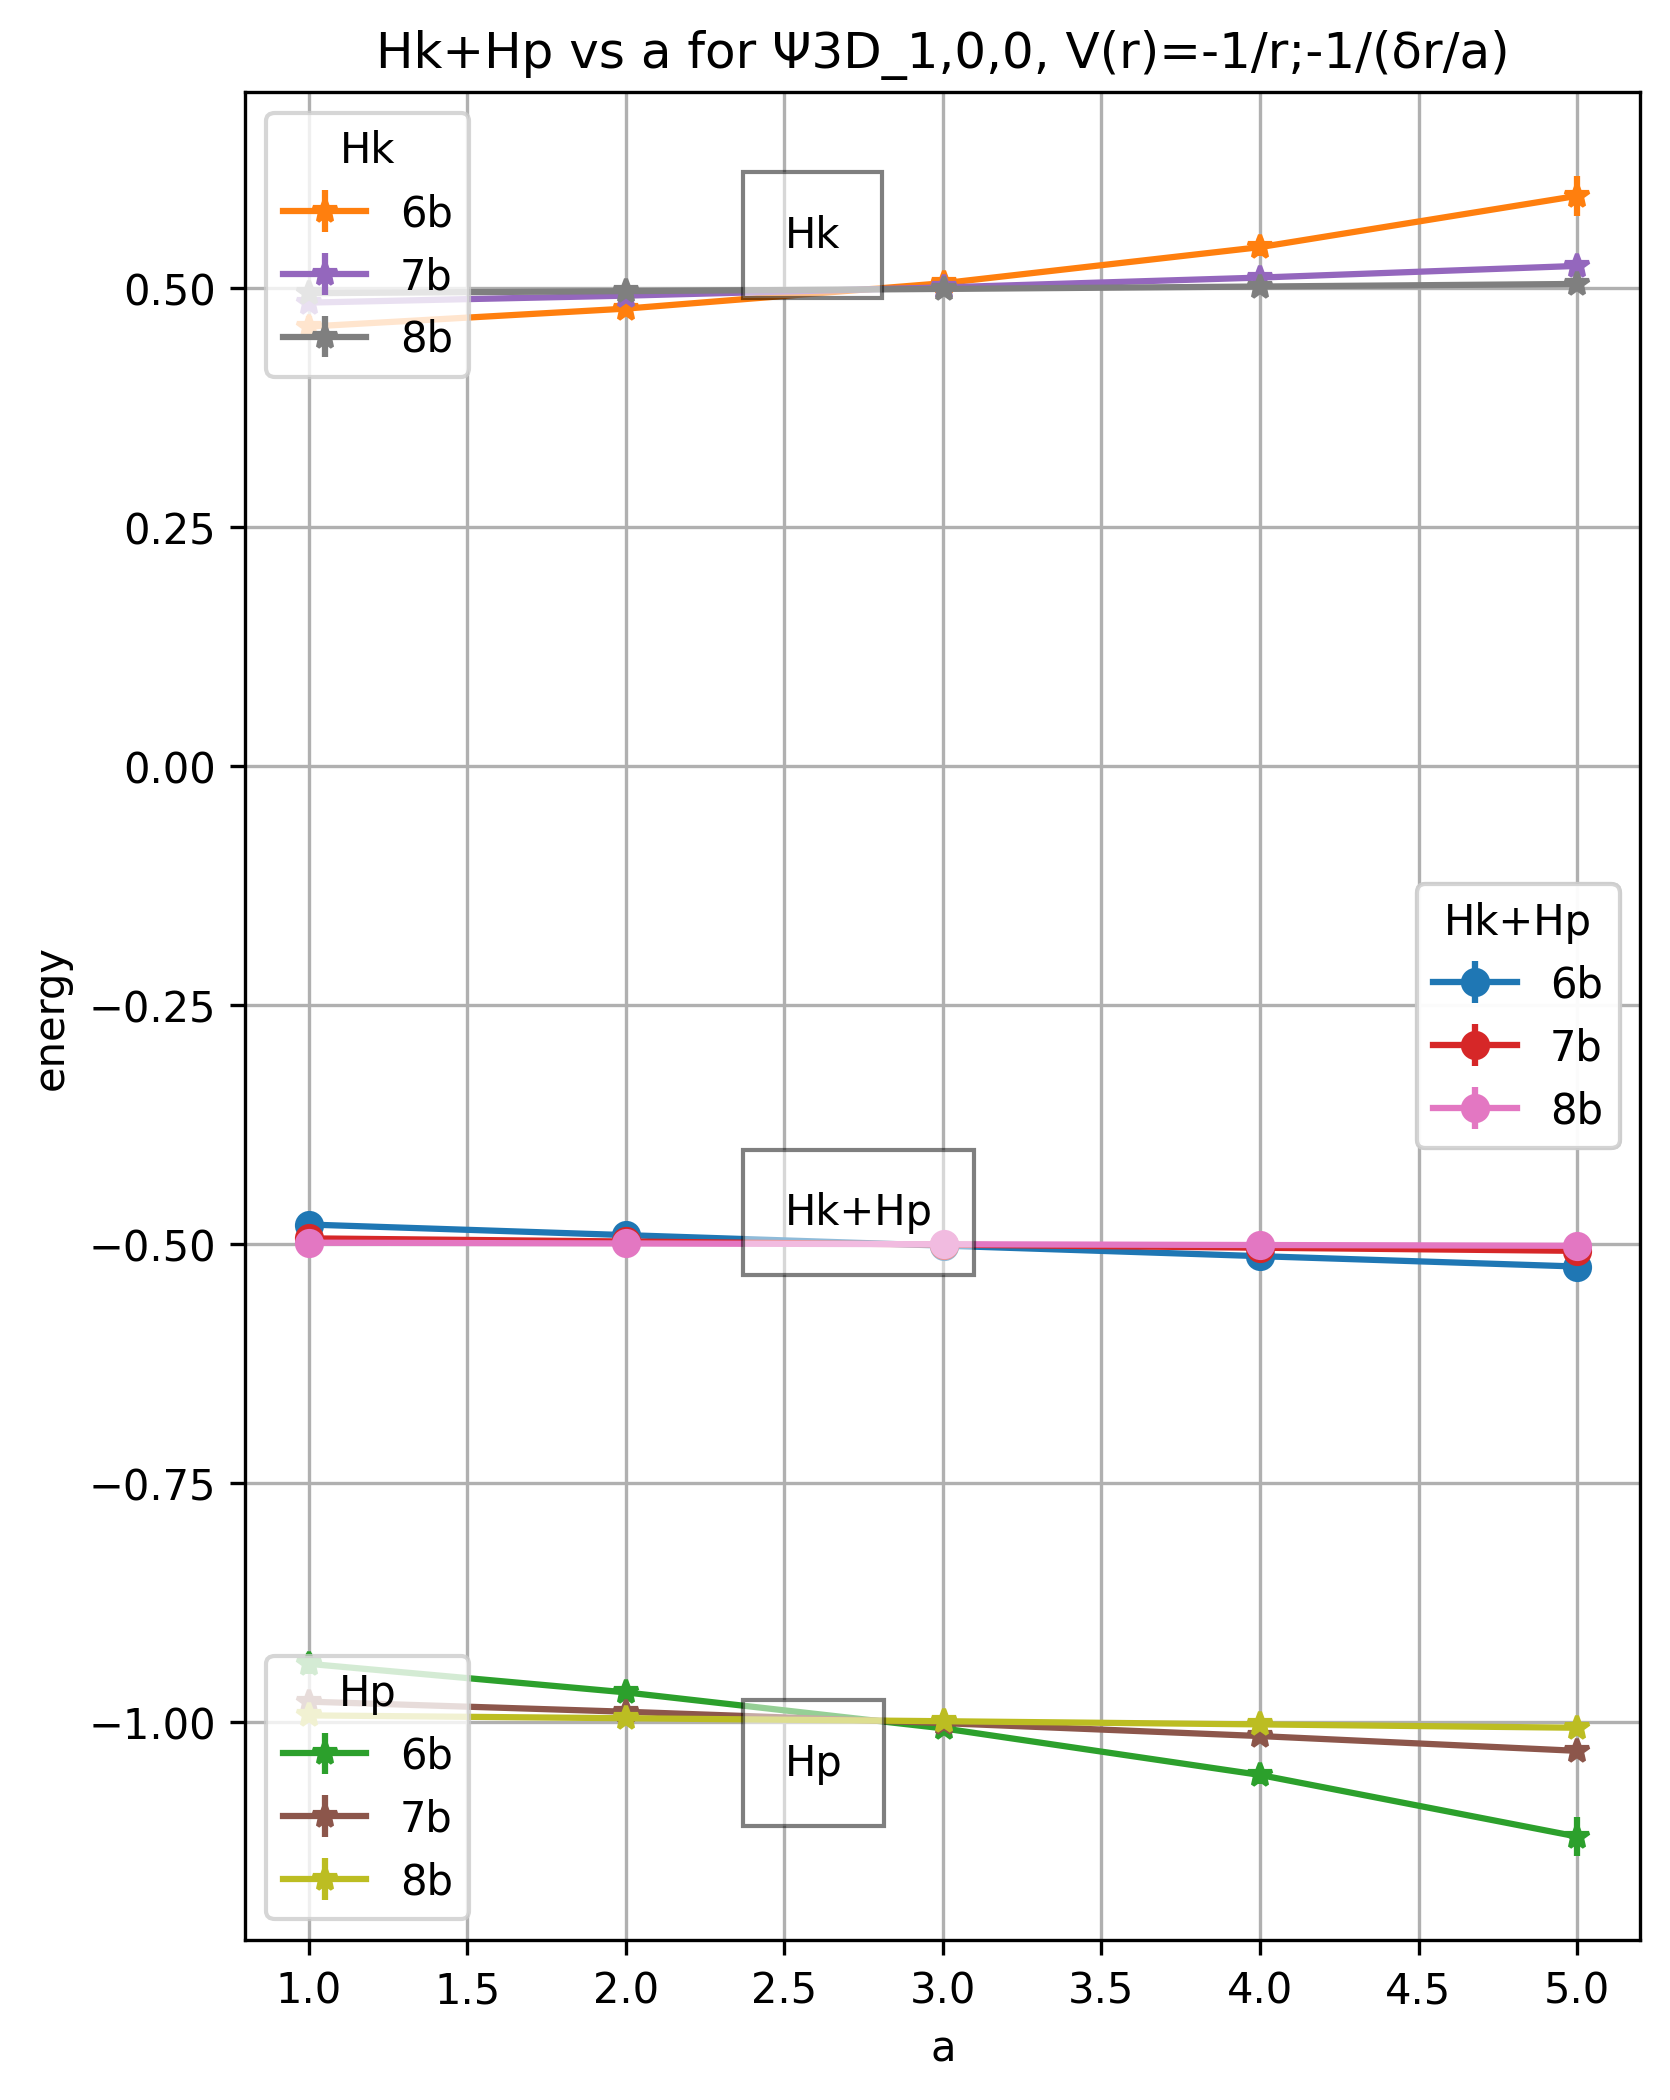
\includegraphics[width=0.6\columnwidth]{paper2025_figs/compare_energy/compare_energy_h3D_TO2_r0lim_1_0_0.png}
    \caption{Changes in energy values when varying $\reff$ in the approximation formula $\Hla(r)$ for the 3D hydrogen atom model}
    \label{fig:Ha1-vs-delta1-3d}
    \begin{flushleft}\small
      
        Graph for the state $\PsiThreeD_{1,0,0}$, setting $\reff=\deltar/a$ and varying $a$. Across all bit counts, the expectation value of the Hamiltonian $\Hk+\Hp$ shows a value close to the analytical solution of $-0.5$ when $a=3$ ($\reff=\deltar/3$).
    \end{flushleft}
\end{figure}

\end{document}
